\section{Results}
\label{Results}
%
The 567 affinity notes were sorted into 149 blue categories, which were then sorted into 47 pink categories, which were finally sorted into 10 green categories. To gain more insight we decided to mix the spontaneous answers from the conversation topics with the answers from the specific questions. These are not differentiated in the affinity diagram. Of the 10 green categories we chose to exemplify four categories which are related to the robot’s appearance (udseende), behaviour (væremåde), approach (henvendelse), and trust (tillid). Based on these categories a variable can be elicitated according to the criterion of a) being changeable and b) the possibility of formulating the variables as a scale question. Because the field study is conducted on Danish speaking test subjects the variables are listed i both English and Danish. For each of the four main categories the following variables can be elicitated and formulated as a scale question:\\
%
\begin{itemize}
\item Appearance 
  \begin{itemize}
  \item I like R's look (Jeg kan godt lide R's udseende)
  \item I think R is elegant (Jeg synes R er elegant)
  \item I prefere a more human-like look (Jeg foretrækker at R ser menneskelig ud)
  \item I think R looks human (Jeg synes R ser menneskelig ud)
  \item I think R's height is (Jeg synes at R's højde er)
\end{itemize}
\item Behaviour
  \begin{itemize}
  \item I think R's speed is (Jeg synes at R's hastighed er)
  \item I think R is alive (Jeg synes R er levende)
  \item I think R's movements are calm (Jeg synes R har rolige bevægelser)
  \item I think R is annoying (Jeg synes R er irriterende)
  \item I think R is intrusive (Jeg synes R er anmassende)
  \item I think R's movements are pleasant (Jeg synes R's bevægelser er behagelig)
\end{itemize}
\item Approach 
\begin{itemize}
  \item I was surprised by R's approach (Jeg blev overrasket over R's henvendelse)
  \item I thought that R was blocking my way (Jeg synes R stod i vejen) 
  \item I prefere to approach R (Jeg foretrækker at jeg henvender mig til R)
  \item I prefere R to approach me (Jeg foretrækker at R henvender sig til mig) 
\end{itemize}
\item Trust
\begin{itemize}
  \item I feel safe around R (Jeg føler mig tryg ved R)
  \item I count on R to follow me to the right place (Jeg regner med at R følger mig hen til det sted jeg har valgt) 
  \item R scared me (R gjorde mig forstrækket)\\
\end{itemize}
\end{itemize}
%
The scale questions can either be presented on a bi- or unipolar \textit{Visual Analoge Scale} (VAS) with open anchor points. If the scale is bipolar a midt point will be marked as shown on \autoref{fig:Height}.
%
\begin{figure}[H]
\centering

\includegraphics[width = 0.49\textwidth]{Figure/HeightHoejde} 
\caption{Example of a bipolar scale relevant for the scale question: \textit{I think R's height is}.}
\label{fig:Height}
\end{figure}
\noindent
% 
An example of a unipolar scale is illustrated on \autoref{fig:HumanMenneskelig}.
%
\begin{figure}[H]
\centering
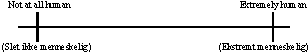
\includegraphics[width = 0.49\textwidth]{Figure/HumanMenneskelig} 
\caption{Example of a unipolar scale relevant for the scale question: \textit{I think R looks human}.}
\label{fig:HumanMenneskelig}
\end{figure}
\noindent
